\secput{cacheoblivious}{Cache-oblivious Tools}

This section describes some cache-oblivious primitive operations that are known
in the literature and useful to build up solutions to the iterated predecessor problem
in this paper.

\subsection*{Array Scanning}
Accessing a random element in an length $n$ array requires $O(1)$ memory
transfers. However, if we access the entire array in order, we can achieve
$O(n/B)$ memory transfers, where $B$ is the size of a block in cache. Each
memory transfer brings $B$ elements into cache, so we must make at most
$O(n/B)$ transfers.

\subsection*{vEB Layout} 
Traditional binary search on an array requires $O(\lg \paren{n/B})$ 
memory transfers. Every access to the array is a random access, and could
be located in a different cache block, except for the last $O(\lg B)$ elements
which are located on the same block.

The vEB layout as depicted in \figref{veb} tries to optimize 
memory transfers by rearranging the array. It
works by recursively dividing the tree into triangles, and storing each
triangle contiguously in memory. This means that children and parent nodes are
likely to be stored together in memory, reducing the number of memory transfers
required.

\begin{figure}[h]
\begin{center}
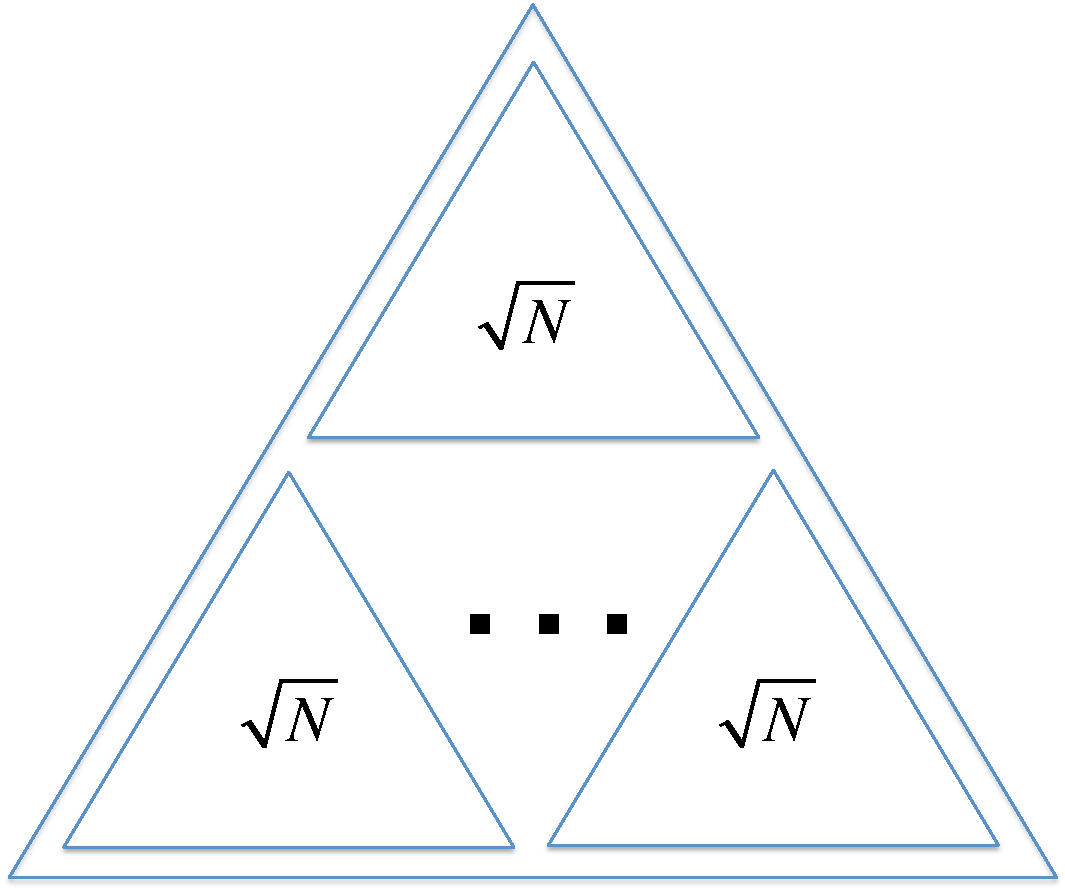
\includegraphics[scale=.35]{veb.pdf}
\end{center}
\caption{vEB trees are recursively divided into triangles of size $\sqrt{N}$. Each of these
triangles is stores contiguously in memory.}
\label{fig:veb} 
\end{figure}

\begin{lemma} 
A query on an binary tree in the vEB layout requires $O(\log_{B+1} n)$
memory transfers. 
\end{lemma}

\begin{proof} 
Triangles of size $M$ are recursively divided into smaller
triangles of size $\sqrt{M}$. Lets examine the largest triangle that has at most
$B$ elements. This triangle must have at least $\sqrt{B+1}$ elements, so its
height must be at least $\frac{1}{2}\lg \paren{B+1}$. This entire triangle can be loaded
into one cache block. There are at most 
$\lg n/ \frac{1}{2}\lg \paren{B+1} = 2 \log_{B+1} n$ 
of these triangles along a root to leaf path, so we only need to make
$O(\log_{B+1} n)$ memory transfers to find an element. 
\end{proof}

The vEB layout has been the basis for several known cache-oblivious algorithms, including 
$B$-trees~\cite{BayerMc72}, funnel sort~\cite{FrigoLePr99}, and priority 
queues~\cite{ArgeBeDe02,BrodalFa02}. It is also used in our solution for range coalescing. 



